\documentclass[a4paper]{article}

\usepackage[utf8]{inputenc}
\usepackage[T1]{fontenc}
\usepackage{amsmath, amssymb, physics, braket, graphicx, subcaption}

\newcommand{\en}{\varepsilon}
\newcommand{\Ha}{\hat{\mathcal{H}}}
\newcommand{\eff}{_{\textnormal{eff}}}
\newcommand{\I}{\hat{I}}

\newcommand{\Sv}{\vec{\sigma}}
\newcommand{\Sp}[1]{\hat{\sigma}^{#1}}

\newcommand{\C}{\hat{a}^{\dagger}}
\newcommand{\D}{\hat{a}}

\newcommand{\Cb}{\hat{b}^{\dagger}}
\newcommand{\Db}{\hat{b}}

\newcommand{\M}[1]{\alpha^{#1}}
\newcommand{\Mb}[1]{\beta^{#1}}

\title{Next nearest neighbor Kitaev Chain/Ring}
\author{Ivo A. Maceira}

\begin{document}
\maketitle
\pagebreak

\section{NNN Kitaev 1D model}
\label{sec:nnn_kitaev_1d_model}
In this notes I discuss the phase diagram of the 1D Kitaev model with next nearest neighbor couplings (NNN). The model is
\begin{equation}
	\Ha = \sum_{l=1}^{2}\sum_{n=1}^{N-l\lambda}( t_l\C_{n}\D_{n+l} + \Delta_l\C_{n}\C_{n+l} + \textrm{H.c.}) + \mu\sum_{n=1}^{N} 2(\C_{n}\D_{n} - 1),
\end{equation}
where $\C_n$ are fermion creation operators, $N$ is the number of lattice sites, $\lambda$ is $0$ (ring) or $1$ (chain), and we take the couplings to be real. A solution of the model will take the form
\begin{equation}
	\Ha = \sum_{k} \en_k (\Cb_k \Db_k - \Db_k \Cb_k),
	\label{eq:H_bogoliubov}
\end{equation}
where $\Cb_k$ is a Bogoliubov quasi-particle and $\en_k$ the associated excitation energy. Our interest is in $\en_k = 0$ solutions of this model.

In the thermodynamic limit ($N \rightarrow \infty$), the chain model has $\en_k = 0$ quasi-particles in some region of the parameter space. These quasi-particles are exponentially localized at the edges of the chain. Let us call the number of $\en_k = 0$ solutions as $\nu$. This quantity is not well defined when the model is gapless. One can show using symmetries of the model that $\nu$ only changes in value when we cross a gapped-gapless-gapped transition by tuning some coupling. Thus $\nu$ can characterize gapped phases.

While the gapped phases of the ring and chain models coincide, in the ring we have no $\en_k = 0$ edge-localized solutions since we have no edges, so $\nu = 0$. However, one can find a winding number $W$ in the ring that will coincide in absolute value with $\nu$ for the chain\footnote{The winding number seems to agree with the number of edge excitations not only for this model but also for more general models with the same symmetries. This suggests a deeper connection between the winding of the band and the edge excitations which I do not understand.}. We shall obtain the phase diagram in the ring since it's much simpler to solve.

\section{Phase diagram on the ring}
\label{sec:phase_diagram_on_the_ring}

Taking the case of the ring, our model is translation invariant, so a transformation to a quasi-momentum basis is appropriate. Our new basis of operator will be given by
\begin{equation}
	\D_k \equiv \sum_{n=1}^{N} e^{i k n} \D_n,
	\label{eq:destruction_operator_momentum}
\end{equation}
where we take the quasi-momentum $k$ to take the values
\begin{equation}
	k \equiv \frac{2\pi l}{N},\quad l=-\frac{N-1}{2},\cdots,\frac{N-1}{2}.
\end{equation}
%
Using the inverse relation of Eq.~(\ref{eq:destruction_operator_momentum}) and appropriately organizing terms, we can write the Hamiltonian as
\begin{equation}
	\label{eq:H_momentum_basis}
	\Ha = \sum_{k}
	\left(\begin{matrix}
		\C_k & \D_{-k}
	\end{matrix}\right)
	\left(\vec{r}_k \cdot \Sv\right)
	\left(\begin{matrix}
		\D_k \\
		\C_{-k}
	\end{matrix}\right),
\end{equation}
where
$
\vec{r}_k \equiv (0,y_k,z_k)
$
with
\begin{equation}
	y_k \equiv \Delta_1 \sin{k} + \Delta_2 \sin{2k},\quad
	z_k \equiv t_1 \cos{k} + t_2 \cos{2k} + \mu,
\end{equation}
and
$
\Sv \equiv (\Sp{x},\Sp{y},\Sp{z})
$
are Pauli matrices. It will be useful to write $\vec{r}_k$ in polar coordinates in the $zy$ plane, with magnitude $\en_k$ and polar angle $\phi_k$ given by
\begin{equation}
	\en_k = \sqrt{z_k^2 + y_k^2},\quad
	\tan{\phi_k} = \frac{y_k}{z_k}.
\end{equation}
Diagonalizing the $2 \times 2$ Hermitian matrix in Eq.~(\ref{eq:H_momentum_basis}), we get
\begin{align}
	y_k \Sp{y} + z_k \Sp{z} &= U^{\dagger} \Sigma U,\\
	U \equiv
	\left(\begin{matrix}
		\cos{\frac{\phi_k}{2}}  & i\sin{\frac{\phi_k}{2}} \\
		i\sin{\frac{\phi_k}{2}} & \cos{\frac{\phi_k}{2}}
	\end{matrix}\right)&,\quad
	\Sigma\equiv
	\left(\begin{matrix}
		\en_k & 0 \\
		0 & -\en_k
	\end{matrix}\right).
\end{align}
Defining the fermionic quasi-particles $\Db_k$ as
\begin{equation}
	\left(\begin{matrix}
		\Db_k \\
		\Cb_{-k}
	\end{matrix}\right)
	\equiv U
	\left(\begin{matrix}
		\D_k \\
		\C_{-k}
	\end{matrix}\right),
\end{equation}
our Hamiltonian can be written in the form of Eq.~(\ref{eq:H_bogoliubov}).

\begin{figure}
	\centering
	\begin{subfigure}{0.32\textwidth}
		\centering
		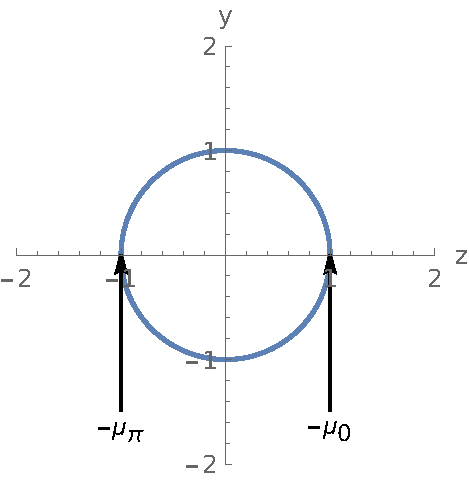
\includegraphics[width=\textwidth]{Figures/r_curve_1.pdf}
		\caption{$t_2 = \Delta_2 = 0$}
		\label{sfig:curve_1}
	\end{subfigure}
	\begin{subfigure}{0.32\textwidth}
		\centering
		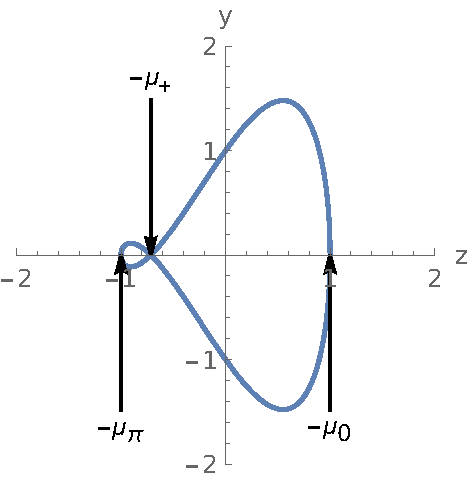
\includegraphics[width=\textwidth]{Figures/r_curve_2.pdf}~
		\caption{$t_2 =0, \Delta_2 = 0.7$}
		\label{sfig:curve_2}
	\end{subfigure}
	\begin{subfigure}{0.32\textwidth}
		\centering
		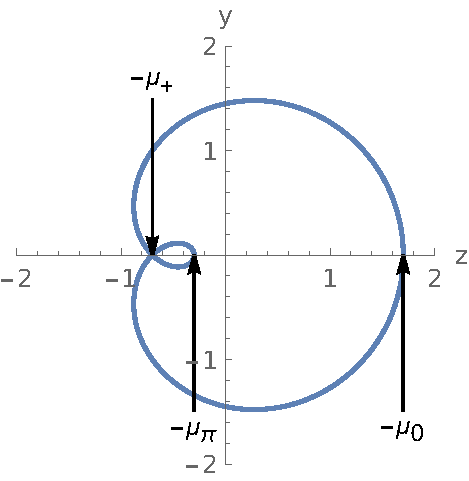
\includegraphics[width=\textwidth]{Figures/r_curve_3.pdf}
		\caption{$t_2 = \Delta_2 = 0.7$}
		\label{sfig:curve_3}
	\end{subfigure}
	\caption{Plot of parametric curves $(z_k,y_k)$ with $-\pi \leq k < \pi$, with parameters $\mu = 0, t_1 = 1, \Delta_1 = 1$. The (absolute) winding number $|W|$ is equal to the number of times the curve winds around the origin. Thus, the three curves have $|W|=1$. Note that $\mu$ causes a translation of this curve along the $z$ axis, so that by adjusting $\mu$ we can cause transitions from $|W|=1$ to $|W|=0$ in (a) and (b), or to $|W|=0,2$ in (c).}
	\label{fig:curves}
\end{figure}

The phases of the open chain model are characterized by the number of zero energy edge excitations present. This quantity coincides or is proportional to the absolute value of the winding number $W$, which is defined in the ring model. The definition is
\begin{equation}
	W \equiv \frac{1}{2\pi} \int_{-\pi}^{\pi} \dv[]{\phi_k}{k} dk = \frac{1}{2\pi} (\phi_{\pi} - \phi_{-\pi}).
\end{equation}
From the second equality we see that $W$ counts how many times the parametrized curve $(z_k,y_k)$ winds around the origin, with (counter)clockwise windings contributing (positively) negatively. Note that the transition points between different windings have an $\en = 0$ solution (gapless).

We will approach the calculation of $W$ as such: we consider that the $t_i,\Delta_i$ parameters are fixed, and we wish to know what phases are realized as we tune $\mu$. We will first determine gapless point of the model, that is,
\begin{align}
	&(z_k,y_k) = (0,0) \Leftrightarrow \\
	&\Leftrightarrow\begin{cases}
		\Delta_1 \sin{k} + \Delta_2 \sin{2k} = 0,\\
		t_1 \cos{k} + t_2 \cos{2k} + \mu = 0.
	\end{cases}
\end{align}
The condition $y_k = 0$ always has $k=0$ and $k=\pi$ as solutions. Two more solutions are possible if
\begin{equation}
	\left|\Delta_1/(2\Delta_2)\right| < 1.
	\label{eq:k_plus_condition}
\end{equation}
They obey
\begin{equation}
	\cos{k_{\pm}} = -\frac{\Delta_1}{2\Delta_2},
\end{equation}
and $k_{-} = - k_{+}$. Substituting these solutions in the $z_k = 0$ condition, and solving for $\mu$, we obtain the following gapless points:
\begin{align}
	k = 0:\quad &\mu_0 = - t_1 - t_2, \\
	k = \pi:\quad &\mu_{\pi} = t_1 - t_2, \\
	k = k_{\pm}:\quad &\mu_{+} = \mu_{-} = t_1\frac{\Delta_1}{2\Delta_2} - t_2 \left[ 2\left(\frac{\Delta_1}{2\Delta_2}\right)^2 - 1 \right],
\end{align}
The points $-\mu_0,-\mu_{\pi},-\mu_{+}$ give us the intersections of the parametric curve with the $z$ axis when $\mu = 0$. While the curve crosses $-\mu_0,-\mu_{\pi}$ once, the point $-\mu_{+}$ is crossed twice, when $k=k_{\pm}$, as one can check in Fig.~\ref{fig:curves}.

The possible phases are determined by the ordering of the points $\mu_0,\mu_{\pi},\mu_{+}$. If $\mu_{+}$ does not exist (Eq.~(\ref{eq:k_plus_condition}) is not satisfied), then there are only two possible phases. Assuming $t_1 > 0$ so that $\mu_{\pi} > \mu_{0}$, we have $|W| = 1$ if $\mu_{0}<\mu<\mu_{\pi}$, and $W = 0$ otherwise. One can check this in Fig.~\ref{sfig:curve_1}.

We take $t_1,t_2>0$, which guarantees that $\mu_0 < \mu_+,\mu_{\pi}$. The last equation we need is
\begin{equation}
	\mu_{\pi} < \mu_{+} \Leftrightarrow \frac{\Delta_1}{2\Delta_2} > \frac{t_1}{2t_2} - 1.
\end{equation}

We summarize the full phase diagram in Table~\ref{tab:phase_diagram}.

\begin{table}
	\centering
	\begin{tabular}{c|c}
		$\left|\frac{\Delta_1}{2\Delta_2}\right|\geq 1$ &
		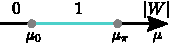
\includegraphics[width=0.4\textwidth]{Figures/phase_diagram_1.pdf} \\
		$\left|\frac{\Delta_1}{2\Delta_2}\right|<1$,
		$\frac{\Delta_1}{2\Delta_2} \leq \frac{t_1}{2t_2} - 1$ &
		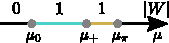
\includegraphics[width=0.4\textwidth]{Figures/phase_diagram_2.pdf} \\
		$\left|\frac{\Delta_1}{2\Delta_2}\right|<1$,
		$\frac{\Delta_1}{2\Delta_2} > \frac{t_1}{2t_2} - 1$ &
		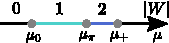
\includegraphics[width=0.4\textwidth]{Figures/phase_diagram_3.pdf} \\
	\end{tabular}
	\caption{Phase diagrams for different parameter ranges. Note that the $|W|=1$ phases in the middle case have opposite windings, as one can check in Fig.~\ref{sfig:curve_2}.}
	\label{tab:phase_diagram}
\end{table}

\bibliographystyle{plain}
\bibliography{$HOME/Docs/bib}

\end{document}
